\documentclass[12pt,twoside]{article}
\usepackage[dvipsnames]{xcolor}
\usepackage{tikz,graphicx,amsmath,amsfonts,amscd,amssymb,bm,cite,epsfig,epsf,url}
\usepackage[hang,flushmargin]{footmisc}
\usepackage[colorlinks=true,urlcolor=blue,citecolor=blue]{hyperref}
\usepackage{amsthm,multirow,wasysym,appendix}
\usepackage{array,subcaption} 
% \usepackage[small,bf]{caption}
\usepackage{bbm}
\usepackage{pgfplots}
\usetikzlibrary{spy}
\usepgfplotslibrary{external}
\usepgfplotslibrary{fillbetween}
\usetikzlibrary{arrows,automata}
\usepackage{thmtools}
\usepackage{blkarray} 
\usepackage{textcomp}
\usepackage[left=0.8in,right=1.0in,top=1.0in,bottom=1.0in]{geometry}

\usepackage{times}
\usepackage{amsfonts}
\usepackage{amsmath}
\usepackage{latexsym}
\usepackage{color}
\usepackage{graphics}
\usepackage{enumerate}
\usepackage{amstext}
\usepackage{blkarray}
\usepackage{url}
\usepackage{epsfig}
\usepackage{bm}
\usepackage{hyperref}
\hypersetup{
    colorlinks=true,
    linkcolor=blue,
    filecolor=magenta,      
    urlcolor=blue,
}
\usepackage{textcomp}
\usepackage[left=0.8in,right=1.0in,top=1.0in,bottom=1.0in]{geometry}
\usepackage{mathtools}
\usepackage{minted}


%% Probability operators and functions
%
% \def \P{\mathrm{P}}
\def \P{\mathrm{P}}
\def \E{\mathrm{E}}
\def \Var{\mathrm{Var}}
\let\var\Var
\def \Cov {\mathrm{Cov}} \let\cov\Cov
\def \MSE {\mathrm{MSE}} \let\mse\MSE
\def \sgn {\mathrm{sgn}}
\def \R {\mathbb{R}}
\def \C {\mathbb{C}}
\def \N {\mathbb{N}}
\def \Z {\mathbb{Z}}
\def \cV {\mathcal{V}}
\def \cS {\mathcal{S}}
\DeclareMathOperator*{\argmin}{arg\,min}
\DeclareMathOperator*{\argmax}{arg\,max}
\newcommand{\red}[1]{\textcolor{red}{#1}}
\newcommand{\blue}[1]{\textcolor{blue}{#1}}
\newcommand{\green}[1]{\textcolor{ForestGreen}{ #1}}
\newcommand{\fuchsia}[1]{\textcolor{RoyalPurple}{ #1}}

%
%% Probability distributions
%
%\def \Bern    {\mathrm{Bern}}
%\def \Binom   {\mathrm{Binom}}
%\def \Exp     {\mathrm{Exp}}
%\def \Geom    {\mathrm{Geom}}
%\def \Norm    {\mathcal{N}}
%\def \Poisson {\mathrm{Poisson}}
%\def \Unif    {\mathrm {U}}
%
\newcommand{\bdb}[1]{\textcolor{red}{#1}}

\newcommand{\ml}[1]{\mathcal{ #1 } }
\newcommand{\wh}[1]{\widehat{ #1 } }
\newcommand{\wt}[1]{\widetilde{ #1 } }
\newcommand{\conj}[1]{\overline{ #1 } }
\newcommand{\rnd}[1]{\tilde{ #1 } }
\newcommand{\rv}[1]{ \rnd{ #1}  }
\newcommand{\rx}{\rnd{ x}  }
\newcommand{\ry}{\rnd{ y}  }
\newcommand{\ra}{\rnd{ a}  }
\newcommand{\rb}{\rnd{ b}  }
\newcommand{\rpc}{\widetilde{ pc}  }

\def \cnd {\, | \,}
\def \Id { I }
\def \J {\mathbf{1}\mathbf{1}^T}

\newcommand{\op}[1]{\operatorname{#1}}
\newcommand{\setdef}[2]{ := \keys{ #1 \; | \; #2 } }
\newcommand{\set}[2]{ \keys{ #1 \; | \; #2 } }
\newcommand{\sign}[1]{\op{sign}\left( #1 \right) }
\newcommand{\trace}[1]{\op{tr}\left( #1 \right) }
\newcommand{\tr}[1]{\op{tr}\left( #1 \right) }
\newcommand{\inv}[1]{\left( #1 \right)^{-1} }
\newcommand{\abs}[1]{\left| #1 \right|}
\newcommand{\sabs}[1]{| #1 |}
\newcommand{\keys}[1]{\left\{ #1 \right\}}
\newcommand{\sqbr}[1]{\left[ #1 \right]}
\newcommand{\sbrac}[1]{ ( #1 ) }
\newcommand{\brac}[1]{\left( #1 \right) }
\newcommand{\bbrac}[1]{\big( #1 \big) }
\newcommand{\Bbrac}[1]{\Big( #1 \Big)}
\newcommand{\BBbrac}[1]{\BIG( #1 \Big)}
\newcommand{\MAT}[1]{\begin{bmatrix} #1 \end{bmatrix}}
\newcommand{\sMAT}[1]{\left(\begin{smallmatrix} #1 \end{smallmatrix}\right)}
\newcommand{\sMATn}[1]{\begin{smallmatrix} #1 \end{smallmatrix}}
\newcommand{\PROD}[2]{\left \langle #1, #2\right \rangle}
\newcommand{\PRODs}[2]{\langle #1, #2 \rangle}
\newcommand{\der}[2]{\frac{\text{d}#2}{\text{d}#1}}
\newcommand{\pder}[2]{\frac{\partial#2}{\partial#1}}
\newcommand{\derTwo}[2]{\frac{\text{d}^2#2}{\text{d}#1^2}}
\newcommand{\ceil}[1]{\lceil #1 \rceil}
\newcommand{\Imag}[1]{\op{Im}\brac{ #1 }}
\newcommand{\Real}[1]{\op{Re}\brac{ #1 }}
\newcommand{\norm}[1]{\left|\left| #1 \right|\right| }
\newcommand{\norms}[1]{ \| #1 \|  }
\newcommand{\normProd}[1]{\left|\left| #1 \right|\right| _{\PROD{\cdot}{\cdot}} }
\newcommand{\normTwo}[1]{\left|\left| #1 \right|\right| _{2} }
\newcommand{\normTwos}[1]{ \| #1  \| _{2} }
\newcommand{\normZero}[1]{\left|\left| #1 \right|\right| _{0} }
\newcommand{\normTV}[1]{\left|\left| #1 \right|\right|  _{ \op{TV}  } }% _{\op{c} \ell_1} }
\newcommand{\normOne}[1]{\left|\left| #1 \right|\right| _{1} }
\newcommand{\normOnes}[1]{\| #1 \| _{1} }
\newcommand{\normOneTwo}[1]{\left|\left| #1 \right|\right| _{1,2} }
\newcommand{\normF}[1]{\left|\left| #1 \right|\right| _{\op{F}} }
\newcommand{\normLTwo}[1]{\left|\left| #1 \right|\right| _{\ml{L}_2} }
\newcommand{\normNuc}[1]{\left|\left| #1 \right|\right| _{\ast} }
\newcommand{\normOp}[1]{\left|\left| #1 \right|\right|  }
\newcommand{\normInf}[1]{\left|\left| #1 \right|\right| _{\infty}  }
\newcommand{\proj}[1]{\mathcal{P}_{#1} \, }
\newcommand{\diff}[1]{ \, \text{d}#1 }
\newcommand{\vc}[1]{\boldsymbol{\vec{#1}}}
\newcommand{\rc}[1]{\boldsymbol{#1}}
\newcommand{\vx}{\vec{x}}
\newcommand{\vy}{\vec{y}}
\newcommand{\vz}{\vec{z}}
\newcommand{\vu}{\vec{u}}
\newcommand{\vv}{\vec{v}}
\newcommand{\vb}{\vec{\beta}}
\newcommand{\va}{\vec{\alpha}}
\newcommand{\vaa}{\vec{a}}
\newcommand{\vbb}{\vec{b}}
\newcommand{\vg}{\vec{g}}
\newcommand{\vw}{\vec{w}}
\newcommand{\vh}{\vec{h}}
\newcommand{\vnu}{\vec{\nu}}
\newcommand{\rvnu}{\vc{\nu}}

\newtheorem{theorem}{Theorem}[section]
% \declaretheorem[style=plain,qed=$\square$]{theorem}
\newtheorem{corollary}[theorem]{Corollary}
\newtheorem{definition}[theorem]{Definition}
\newtheorem{lemma}[theorem]{Lemma}
\newtheorem{remark}[theorem]{Remark}
\newtheorem{algorithm}[theorem]{Algorithm}

% \theoremstyle{definition}
%\newtheorem{example}[proof]{Example}
%\declaretheorem[style=definition,qed=$\triangle$,sibling=definition]{example}
%\declaretheorem[style=definition,qed=$\bigcirc$,sibling=definition]{application}

%
%% Typographic tweaks and miscellaneous
%\newcommand{\sfrac}[2]{\mbox{\small$\displaystyle\frac{#1}{#2}$}}
%\newcommand{\suchthat}{\kern0.1em{:}\kern0.3em}
%\newcommand{\qqquad}{\kern3em}
%\newcommand{\cond}{\,|\,}
%\def\Matlab{\textsc{Matlab}}
%\newcommand{\displayskip}[1]{\abovedisplayskip #1\belowdisplayskip #1}
%\newcommand{\term}[1]{\emph{#1}}
%\renewcommand{\implies}{\;\Rightarrow\;}

% My macros

\def\Kset{\mathbb{K}}
\def\Nset{\mathbb{N}}
\def\Qset{\mathbb{Q}}
\def\Rset{\mathbb{R}}
\def\Sset{\mathbb{S}}
\def\Zset{\mathbb{Z}}
\def\squareforqed{\hbox{\rlap{$\sqcap$}$\sqcup$}}
\def\qed{\ifmmode\squareforqed\else{\unskip\nobreak\hfil
\penalty50\hskip1em\null\nobreak\hfil\squareforqed
\parfillskip=0pt\finalhyphendemerits=0\endgraf}\fi}

%\DeclareMathOperator*{\E}{\rm E}
%\DeclareMathOperator*{\argmax}{\rm argmax}
%\DeclareMathOperator*{\argmin}{\rm argmin}
%\DeclareMathOperator{\sgn}{sign}
\DeclareMathOperator{\supp}{supp}
\DeclareMathOperator{\last}{last}
%\DeclareMathOperator{\sign}{\sgn}
\DeclareMathOperator{\diag}{diag}
\providecommand{\abs}[1]{\lvert#1\rvert}
\providecommand{\norm}[1]{\lVert#1\rVert}
\def\vcdim{\textnormal{VCdim}}
\DeclareMathOperator*{\B}{\textbf{B}}

%\DeclarePairedDelimiter\ceil{\lceil}{\rceil}
%\DeclarePairedDelimiter\floor{\lfloor}{\rfloor}

\newcommand{\cX}{{\mathcal X}}
\newcommand{\cY}{{\mathcal Y}}
\newcommand{\cA}{{\mathcal A}}
\newcommand{\ignore}[1]{}
\newcommand{\bi}{\begin{itemize}}
\newcommand{\ei}{\end{itemize}}
\newcommand{\be}{\begin{enumerate}}
\newcommand{\ee}{\end{enumerate}}
\newcommand{\bd}{\begin{description}}
\newcommand{\ed}{\end{description}}
\newcommand{\h}{\widehat}
\newcommand{\e}{\epsilon}
\newcommand{\mat}[1]{{\mathbf #1}}
%\newcommand{\R}{\mat{R}}
\newcommand{\0}{\mat{0}}
\newcommand{\M}{\mat{M}}

\newcommand{\D}{\mat{D}}
\renewcommand{\r}{\mat{r}}
\newcommand{\x}{\mat{x}}
\renewcommand{\u}{\mat{u}}
\renewcommand{\v}{\mat{v}}
\newcommand{\w}{\mat{w}}
\renewcommand{\H}{\text{0}}
\newcommand{\T}{\text{1}}
%\newcommand{\set}[1]{\{#1\}}
\newcommand{\xxi}{{\boldsymbol \xi}}
\newcommand{\ssigma}{{\boldsymbol \sigma}}
\newcommand{\Alpha}{{\boldsymbol \alpha}}
\newcommand{\tts}{\tt \small}
\newcommand{\hint}{\emph{hint}}
\newcommand{\matr}[1]{\bm{#1}}     % ISO complying version
\newcommand{\vect}[1]{\bm{#1}} % vectors

%\newcommand{\Var}{\mathrm{Var}}
%\newcommand{\Cov}{\mathrm{Cov}}

% New commands
\newcommand{\SP}{\mathbf{S}_{+}^n}
\newcommand{\Proj}{\mathcal{P}_{\mathcal{S}}}
\DeclarePairedDelimiterX{\inp}[2]{\langle}{\rangle}{#1, #2}
\newtheorem{proof}{Proof}


\begin{document}

\begin{center}
{\large{\textbf{Homework 7}} } \vspace{0.2cm}\\
Due April 12 at 11 pm
\end{center}
Yves Greatti - yg390\\

\begin{enumerate}

\item (Fourier coefficients and smoothness) Let $x:\R\to\C$ be
  periodic with period $1$
  and let $\hat{x}[k]$ denote the $k$th Fourier coefficient of $x$,
  for $k\in\Z$ (computed on any interval of length $1$).
  \begin{enumerate}
  \item Suppose $x$ is continuously differentiable. Prove that for
    $k\neq 0$ we have
    $$|\hat{x}[k]| \leq \frac{C_1}{|k|}$$
    for some $C_1\geq0$ that depends on $x$ (but not on $k$). [Hint:
      Integration by parts.  Also note that
      $$\left|\int_0^1 f(t)\,dt\right| \leq \int_0^1 |f(t)|\,dt<\infty$$
    if $f$ is continuous on $[0,1]$.]\\
    
   WLOG we consider the interval [0,1] since  $x$ is periodic with period $1$ and, we have for $k \neq 0$:
    \begin{align*}
	    \hat{x}[k] 	&= \int_0^1 x(t) \exp \brac{- i2 \pi k t}  \diff{t}  \; (\text{by parts with } u=x(t) \text{, and } v=\frac{-1}{i 2 \pi k} e^{-i2 \pi kt})\\	
	    			&= \frac{-1}{i 2 \pi k} [x(t) e^{-i2 \pi kt}]_0^1 + \frac{1}{i 2 \pi k} \int_0^1 x'(t) \exp \brac{- i2 \pi k t}  \diff{t}\\  	
				&=  \frac{x(0) - x(1)} {i 2 \pi k} + \frac{1}{i 2 \pi k} \int_0^1 x'(t) \exp \brac{- i2 \pi k t}  \diff{t}\\
				&=  \frac{1}{i 2 \pi k} \int_0^1 x'(t) \exp \brac{- i2 \pi k t}  \diff{t} \text{ ~ since period is 1 }\\
    \end{align*}
    
    $x$ is continuously differentiable on $[0,1]$ so:
     $$\left|\int_0^1 x'(t)\,dt\right| \leq \int_0^1 |x'(t)|\,dt<\infty$$
     Let  $M=\int_0^1 |x'(t)|\,dt$, using the previous expression of $\hat{x}[k] $, we can now determine an upper bound:
     \begin{align*}
	   | \hat{x}[k]| 	&= |\frac{1}{i 2 \pi k} \int_0^1 x'(t) \exp \brac{- i2 \pi k t}  \diff{t}| \\
	   			&= |\frac{1}{i 2 \pi k}| | \int_0^1 x'(t) \exp \brac{- i2 \pi k t}  \diff{t} | \\
				&\le |\frac{1}{2 \pi k}|  \int_0^1 | x'(t) \exp \brac{- i2 \pi k t}| \diff{t}  \\
				&= |\frac{1}{2 \pi k}|  \int_0^1 | x'(t)  |  |\exp \brac{- i2 \pi k t}| \diff{t}  \\
				&=  |\frac{1}{2 \pi k}|  \int_0^1 | x'(t) |  \diff{t}  \\
				&\le  |\frac{1}{2 \pi k}| M\\
     \end{align*}
     So  $| \hat{x}[k]| \leq \frac{C_1}{|k|}$ with $C_1 = \frac{M}{2 \pi}$.
	         
  \item Suppose $x$ is twice continuously differentiable.
    Prove that for $k\neq 0$ we have
    $$|\hat{x}[k]| \leq \frac{C_2}{|k|^2}$$
    for some $C_2\geq0$ that depends on $x$ (but not on $k$).
    
    Let $ \hat{x}'[k] =  \int_0^1 x'(t) \exp \brac{- i2 \pi k t}  \diff{t}$, using part a, we can write that
    $$\hat{x}'[k] =  \frac{x'(0) - x'(1)} {i 2 \pi k} + \frac{1}{i 2 \pi k} \int_0^1 x''(t) \exp \brac{- i2 \pi k t}  \diff{t}$$ 
    $x$ is now twice continuously differentiable:
     $$\left|\int_0^1 x''(t)\,dt\right| \leq \int_0^1 |x''(t)|\,dt = M_2<\infty$$
     And since $x'$ is continuous on $[0,1]$, it is bounded, let $M_1 = \max|x(t)|, t \in [0,1]$ then
      \begin{align*}
	   | \hat{x}'[k]| 	&\le \frac{|x'(0) | +  |x'(1) |} {|2 \pi k|} +  \frac{1}{|2 \pi k|} M_2\\
	   			&= \frac{2 \; M_1 + M_2} {|2 \pi k|} \\
	  | \hat{x}[k]| 	&= |\frac{1}{i 2 \pi k}| | \int_0^1 x'(t) \exp \brac{- i2 \pi k t}  \diff{t}| \text{ ~ from part a}\\
	  			&\le \frac{C_2} {|k^2|} \text{ ~ where } C_2 = \frac{2 M_1 + M2} {4 \pi^2}
        \end{align*}
    
  \end{enumerate}
  
\newpage

\item (Sampling a sum of sinusoids) We are interested in a signal $x$ belonging to the unit interval $[0,1]$ of the form
\begin{align}
x(t) := a_1 \exp (i 2 \pi k_1 t ) + a_2 \exp (i 2 \pi k_2 t ),
\end{align}
where the amplitudes $a_1$ and $a_2$ are complex numbers, and the
frequencies $k_1$ and $k_2$ are known integers.
We sample the signal at $N$ equispaced locations $0$, $1/N$, $2/N$,
\ldots, $(N-1)/N$, for some positive integer $N$.  
\begin{enumerate}
\item What value of $N$ is required by the Sampling Theorem to
  guarantee that we can reconstruct $x$ from the samples? \\
  
 By theorem 3.4, if the number of samples $N$ is larger than $2 \max{(k_1, k_2)} + 1$ then  the Fourier coefficients $a_1,  a_2$ and hence the signal $x$ can
 be reconstructed. 
 
\item Write a system of equations in matrix form mapping the
  amplitudes $a_1$ and $a_2$ to the samples $x_{N}$. 
  
  $$\MAT{x(\frac{0}{N}) \\ x(\frac{1}{N}) \\ \ldots \\ x(\frac{j}{N}) \\ \ldots\\ x(\frac{N-1}{N}) } 
  	= \MAT{1  & 1 \\  \exp (\frac{i 2 \pi k_1 1} {N} ) & \exp (\frac{i 2 \pi k_2 1} {N} )
	 \\ \ldots &  \ldots \\    \exp (\frac{i 2 \pi k_1 j} {N} ) & \exp (\frac{i 2 \pi k_2 j} {N} ) 
	 \\  \ldots &  \ldots \\    \exp (\frac{i 2 \pi k_1 (N-1)} {N} ) & \exp (\frac{i 2 \pi k_2 (N-1)} {N} ) }
	 \MAT{a_1 \\ a_2 }$$
  
  \item Under what condition on $N$, $k_1$ and $k_2$ can we recover the
  amplitudes from the samples by solving the system of equations? 
  Can $N$ be smaller than the value dictated by the Sampling Theorem?
  If yes, give an example. If not, explain why.  \\
  It is a system of $N$ equations of two unknowns $a_1$ and $a_2$ which has a solution if $N > = 2$ assuming the matrix is at least of column rank $2$ which is
  the case if $k_1 \neq k_2$. If N is smaller that the value dictated by the Sampling Theorem, we may encounter the issue of aliasing for a sinusoid with frequency $m$ such that $m =  \max{(k_1, k_2)} \mod N$,
  the two signals from the samples are indistinguishable.
  
  \item What is the limitation of this approach, which could make it unrealistic?\\
  If we have too many equations, the cost of solving this system using a method like least square will be very costly (in practice with OLS we are looking for a solution of the form $[a_0 a_1]^T = (A A^T )^{-1} A$ where $A$ is the two columns matrix defined in
  part b, this will requires a time proportional at least to $\mathcal{O}(N^3$), making large problem signal reconstruction intractable. In addition solving this system with the matrix $A$ can be prone to machine errors 
  not only when $N$ is large but also when $k_1 \approx k_2$.
  
\end{enumerate}
   
\newpage
   
\item (Sampling theorem for bandpass signals) Bandpass signals are signals that have nonzero Fourier coefficients
only in a fixed band of the frequency domain. We are interested in
sampling a bandpass signal $x$ belonging to the unit interval $[0,1]$
that has nonzero Fourier-series coefficients between $k_1$ and $k_2$,
inclusive, where $k_1$ and $k_2$ are known positive integers such that $k_2 > k_1$. 
\begin{enumerate}
\item We sample the signal at $N$ equispaced locations $0$, $1/N$, $2/N$, \ldots, $(N-1)/N$. What value of $N$ is required by the Sampling Theorem to guarantee that we can reconstruct $x$ from the samples?\\
The minimum value of $N$ required by the Sampling theorem is $N \ge 2 k_2 + 1$.

\item Assume that $k_2:=k_1 + 2\tilde{k}_c$, where $\tilde{k}_c $ is a positive integer. For any $N \geq 2\tilde{k}_c + 1$ it is possible to recover the signal from the samples. Explain why (you don't need to derive any explicit expressions).\\
If  $k_2:=k_1 + 2\tilde{k}_c$ then $N \geq 2\tilde{k}_c + 1$ means that $N \geq k_2 - k_1$. Knowing that the signal has nonzero Fourier-series coefficients only between $k_1$ and $k_2$, there could be only at most $k_2 - k_1 + 1$ nonzero
coefficients in the interval $[k_1, k_2]$, having the number of samples $N \ge k_2 - k_1 + 1$ allows to recover fully the $k_2 - k_1 + 1$ Fourier coefficients hence the original signal $x$.

\item Assume that $k_2:=k_1 + 2\tilde{k}_c$, $N\geq 2\tilde{k}_c+1$,
  and $mN = k_1+\tilde{k}_c$ for some integer $m$. Explain precisely how to recover $x$ from the samples in this case.
 Since   $N\geq 2\tilde{k}_c+1$, from the previous question we know that we can take $N$ samples of $x$ in [0,1] and find all the Fourier coefficients between $[k_1, k_2]$. 
 In addition $k_2:=k_1 + 2\tilde{k}_c$ or $\tilde{k}_c = \frac{k_2 - k_1}{2}$ and $mN=k_1 + \tilde{k}_c = \frac{k_1 + k_2}{2}$.
 From $mN$ we find the point in the frequency domain $\frac{k_1 + k_2}{2}$ and we sample $N$ points of $x$ from the frequency $\frac{k_1 + k_2}{2} - \tilde{k}_c = k_1$ to the frequency $\frac{k_1 + k_2}{2} + \tilde{k}_c = k_2$:
 The Fourier coefficients of the signal can be recovered from $N$ samples where:
 \begin{align*}
 	x(\frac{j\; T}{N})	&= \sum_{k=-\tilde{k}_c}^{k=\tilde{k}_c}  \hat{x}[k]  \exp (\frac{i 2 \pi k j} {N}) \\
 \end{align*}
 
  	\begin{figure}[H]
		\centering
		\captionsetup{justification=centering}
		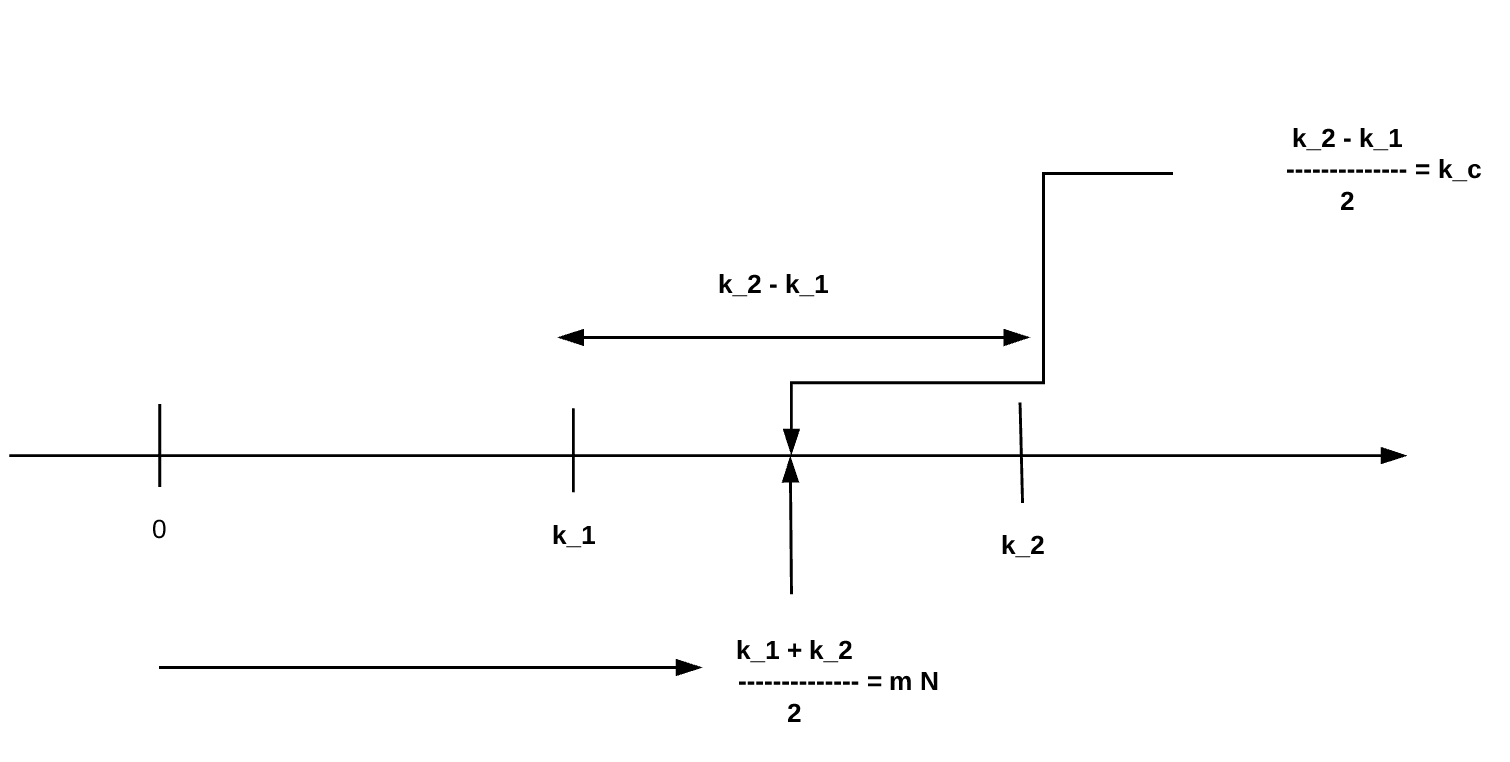
\includegraphics[width=200pt]{Q3_c.png}
	\end{figure}


\end{enumerate} 
 
 \newpage
 \item  (Frequency analysis of musical notes) In this exercise you will
  use the code and data in the \texttt{musicdata} folder.  Make sure you have
  the python packages sklearn, pandas, sounddevice, and soundfile
  installed.  The skeleton code for you to work with is given in
  \texttt{analysis.py} which uses tools given in
  \texttt{music\_tools.py}.  The data used here comes from the NSynth
  dataset.

  \begin{enumerate}
  \item Plot the audio signals for the first signal in the training
    set, and the first vocal signal in the training set (i.e., the
    first signal whose \texttt{instrument\_family\_str} field is
    'vocal' in the dataframe).  In the titles of your two plots, include the
    \texttt{instrument\_family\_str} and the frequency (in Hz).
    We recommend you also use \texttt{play\_signal}
    to hear what the signals sound like.
    
	\begin{figure}[H]
		\centering
		\captionsetup{justification=centering}
		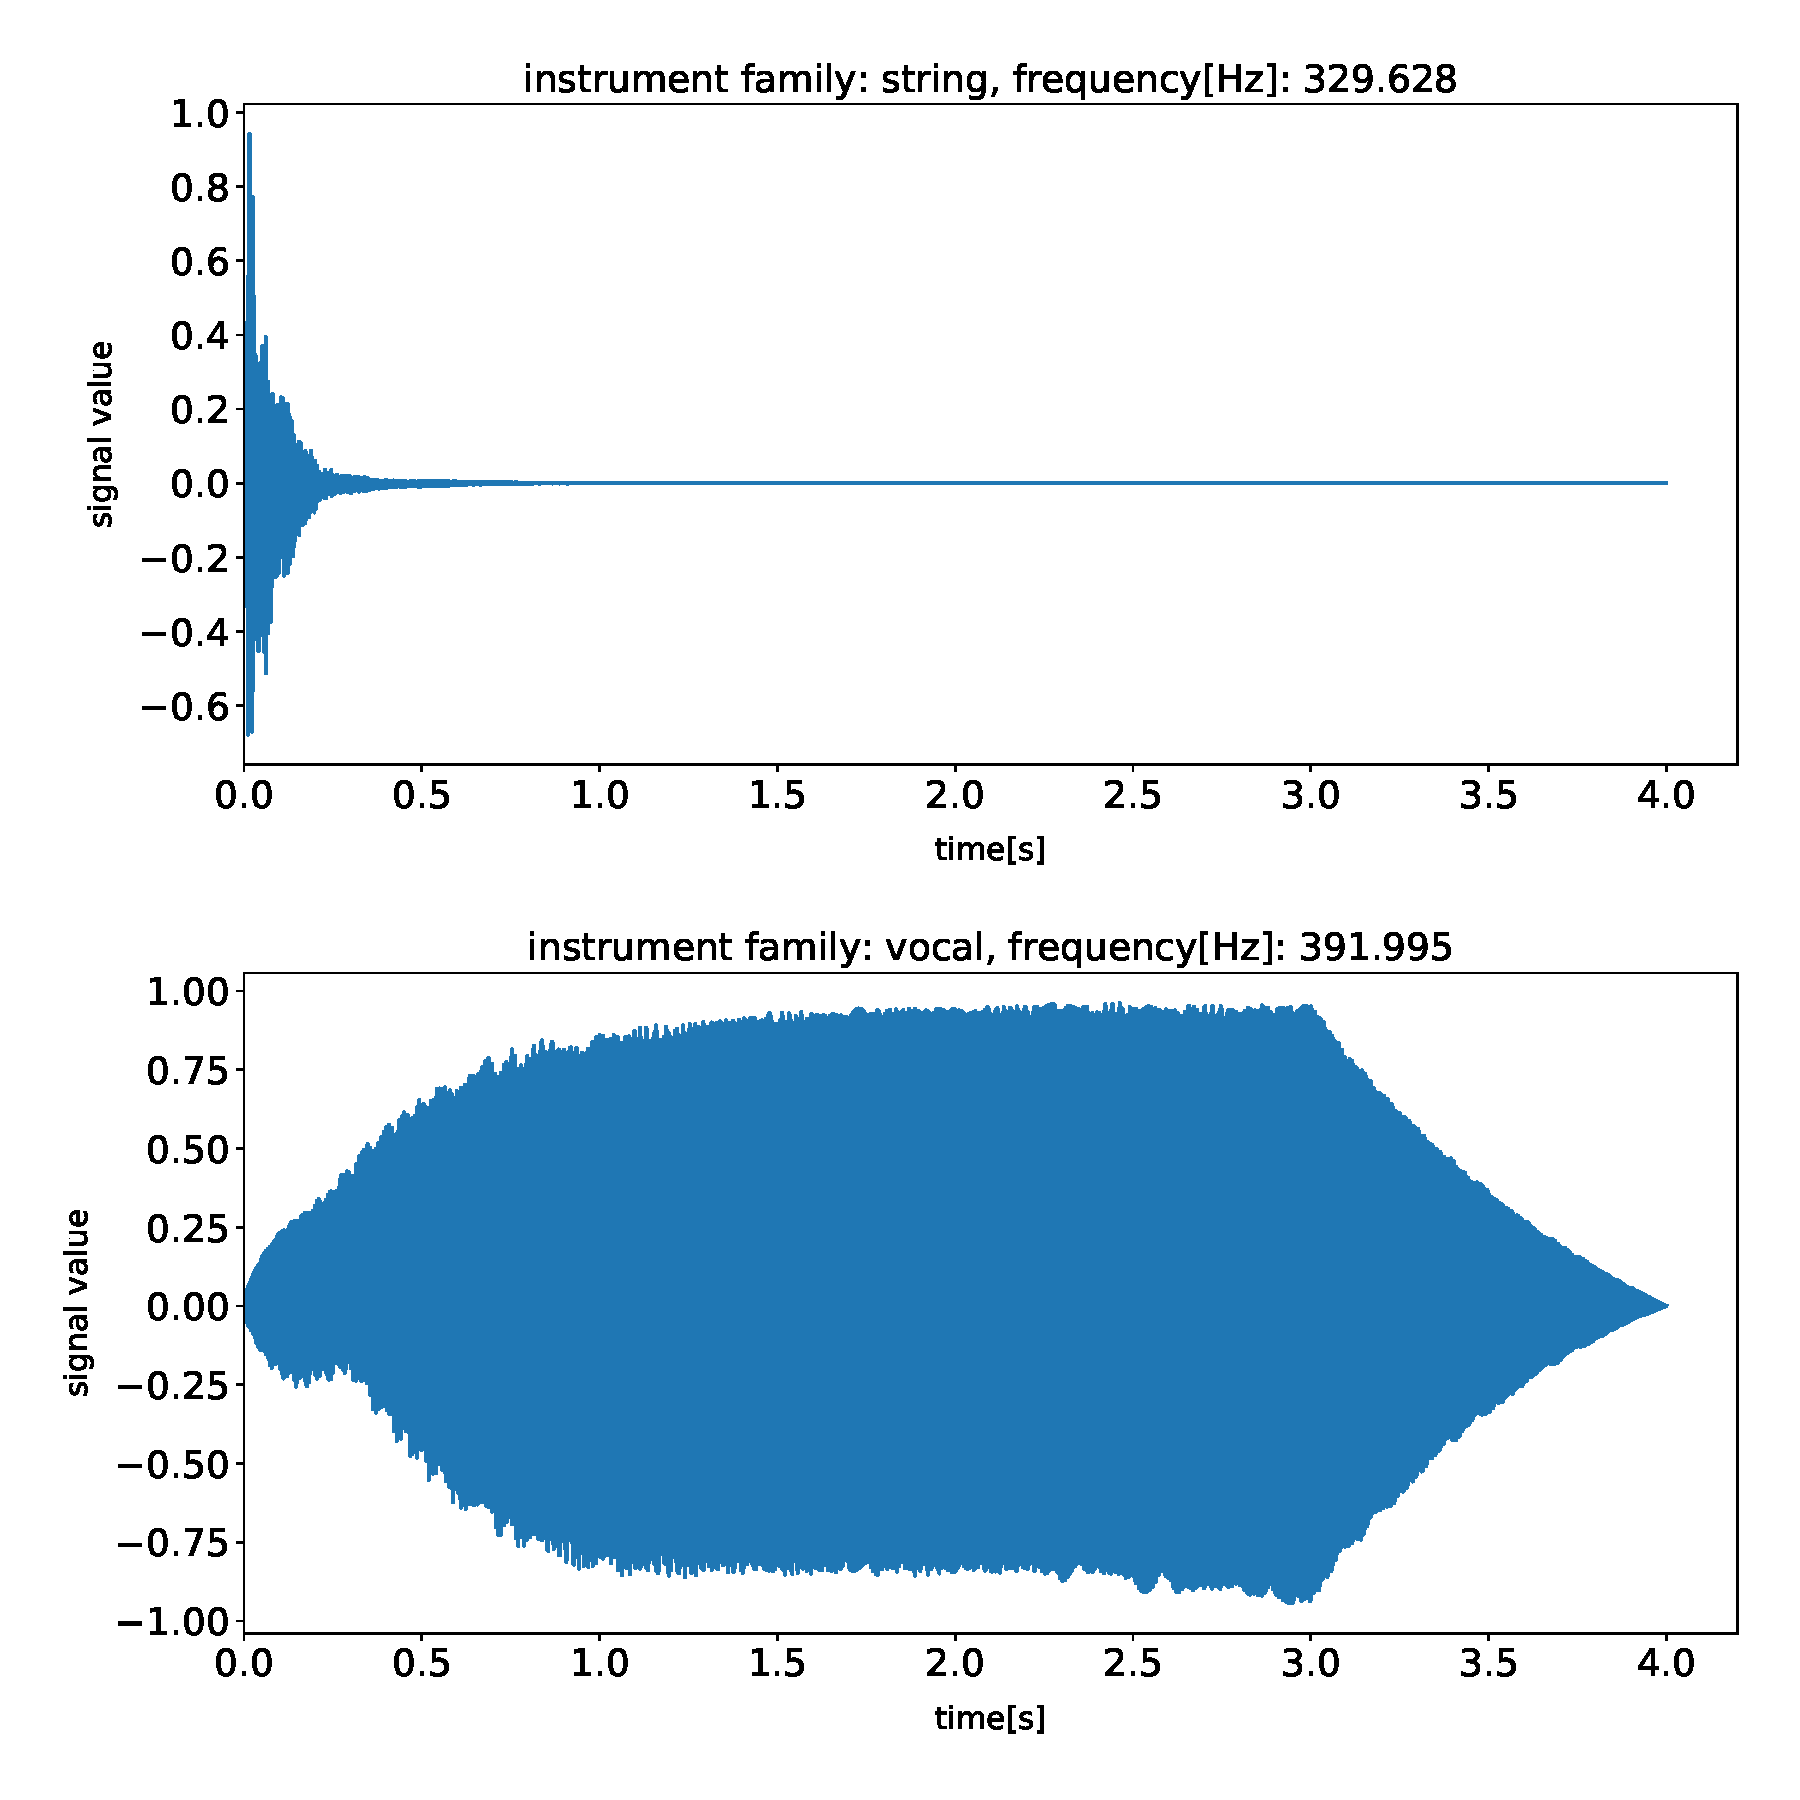
\includegraphics[width=200pt]{code/musicdata/signals.pdf}
		\caption{First signal and first vocal signal in the training set.}
		%\label{simplemodel}
	\end{figure}

    
  \item For each signal in the test set, compute the (strictly positive)
    frequency with the largest amplitude (in absolute value), and
    convert it to a pitch number (using the tools in
    \texttt{music\_tools}).  This will be our predicted pitch.
    \begin{enumerate}
    \item Report what overall fraction of the signals in
      the test set you accurately predict using this method (i.e.,
      your overall accuracy).\\
      Using this method, the overall accuracy obtained is: $72.084\%$.
    \item For the
      first two signals you misclassify (in the order they occur in the
      test set), give plots of their absolute
      DFT coefficients (use \texttt{np.fft.fft} and make one plot per
      signal). In the title of your plots, include the
      \texttt{instrument\_family\_str}, the true frequency, and the
      predicted frequency (in Hz).  Make
      sure to plot the coefficients on an axis centered at $0$ by using
      fftfreq with the correct arguments.\\
      
	\begin{figure}[H]
		\centering
		\captionsetup{justification=centering}
		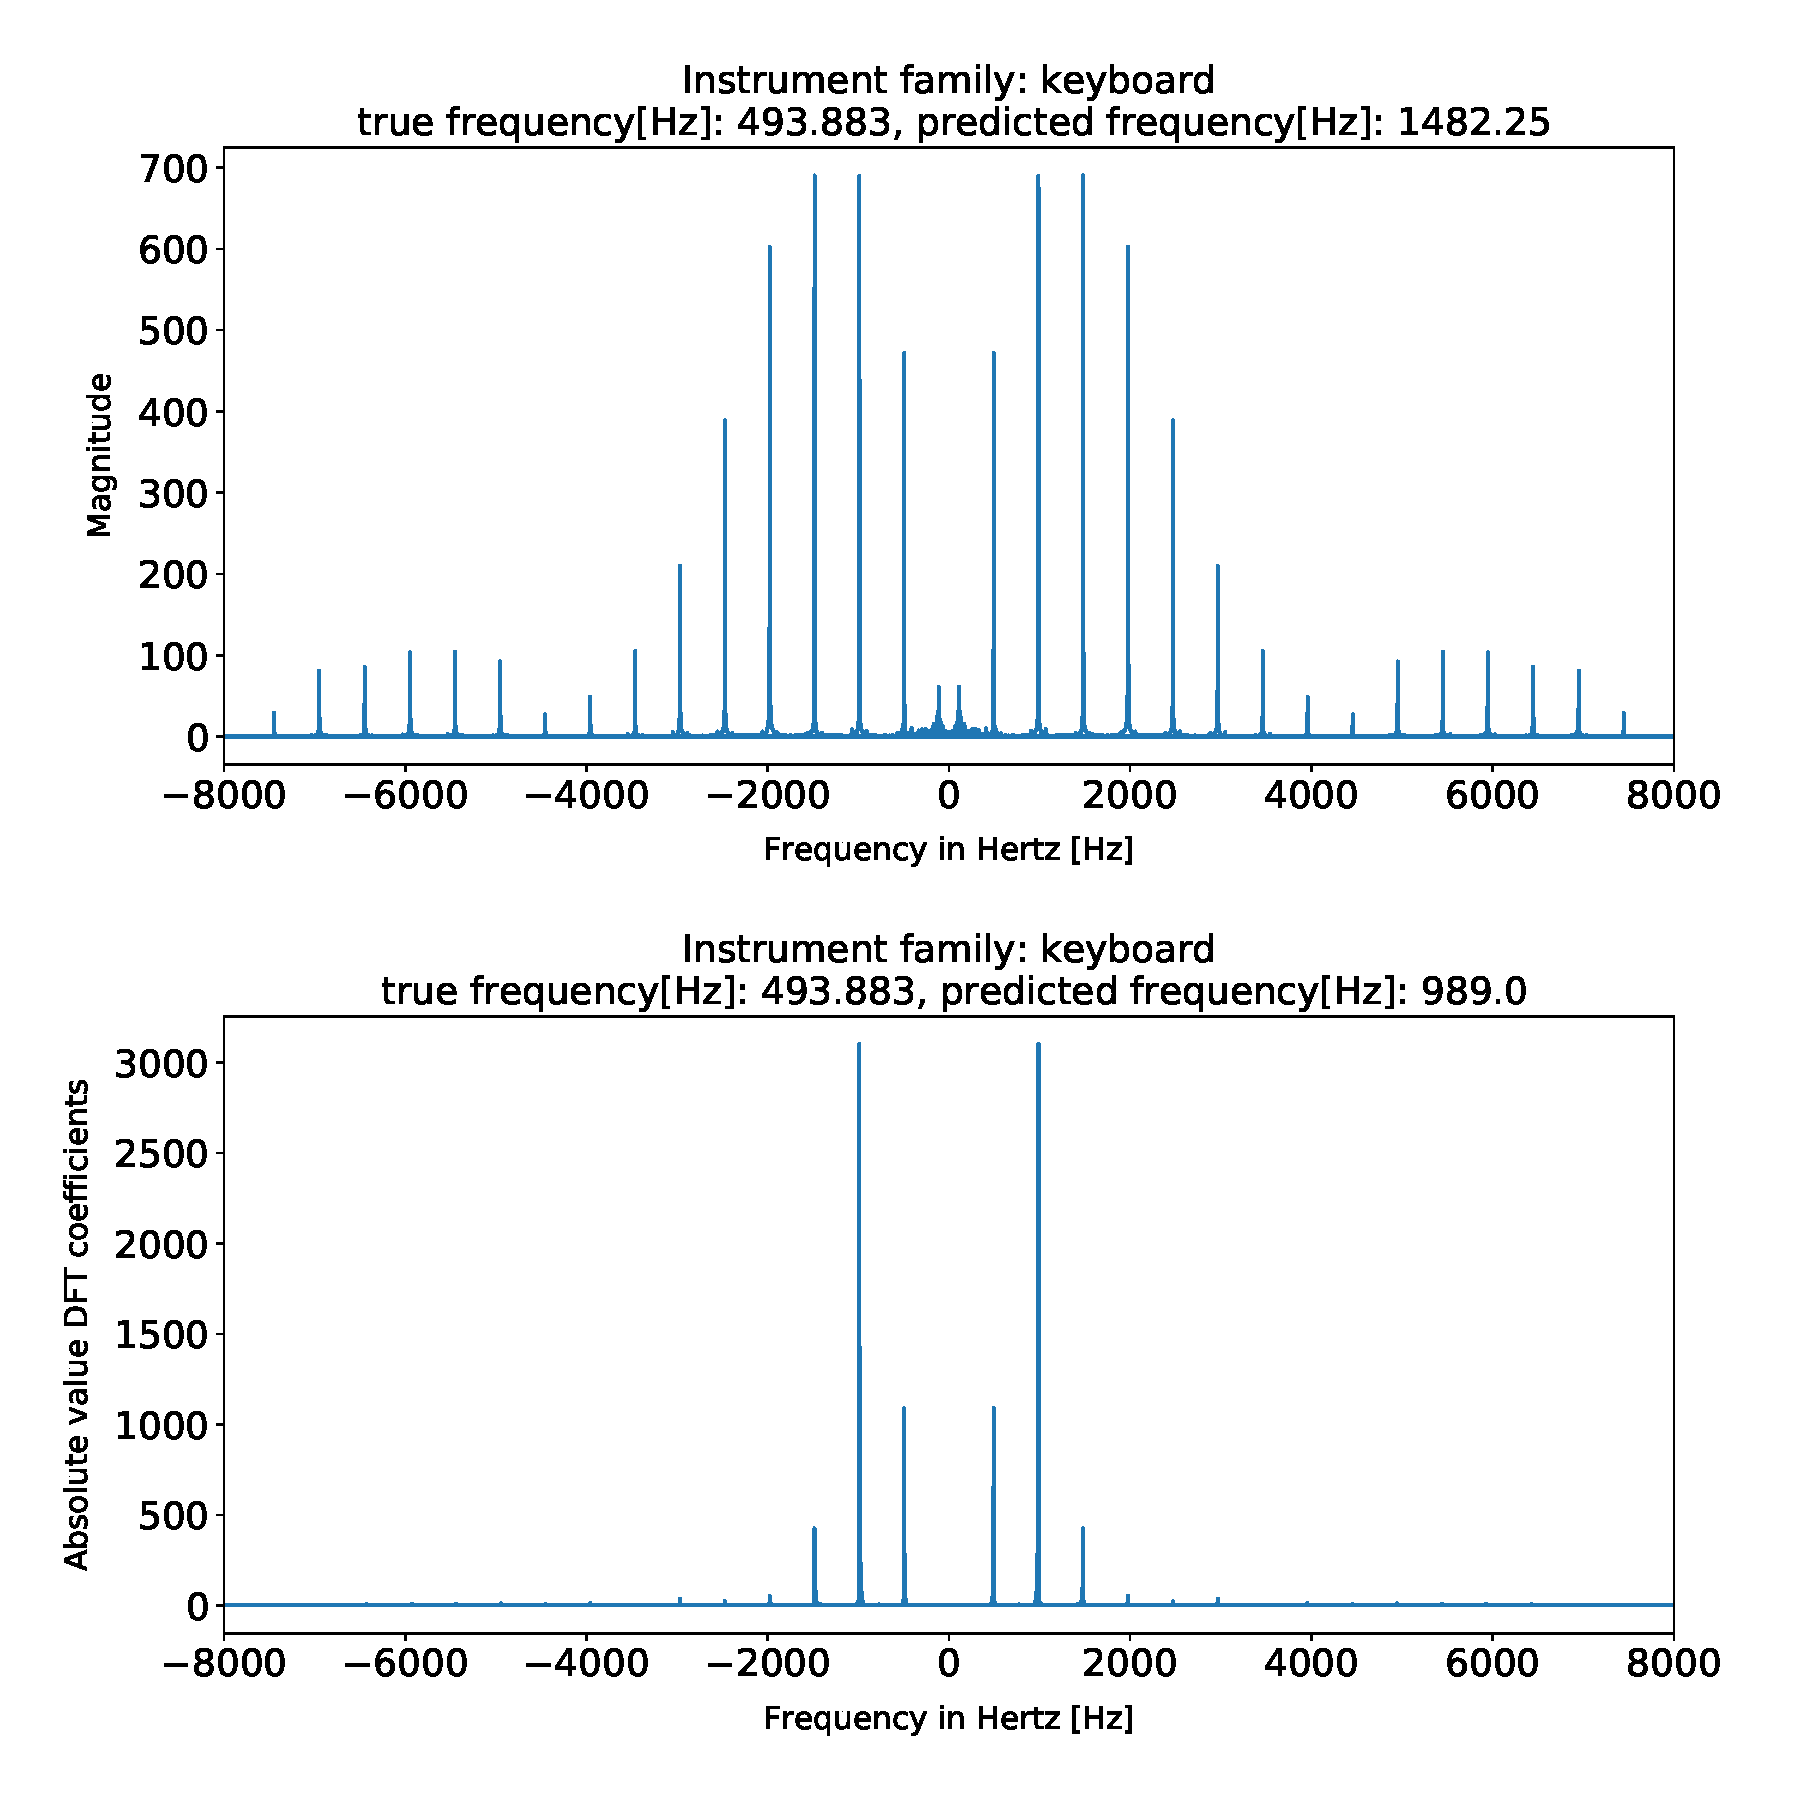
\includegraphics[width=200pt]{code/musicdata/misclassified_signals.pdf}
		\caption{First signal and second misclassified signals in the test set.}
	\end{figure}

      
    \item What is the instrument family for which the method got the
      highest fraction of incorrect predictions (i.e., number incorrect
      divided by number of examples from that family)?
      The instrument family with the highest fraction of incorrect predictions is the family $10$ which corresponds
      to the vocal instrument\_family\_str.
      
    \end{enumerate}
  \item Use the \texttt{LogisticRegression} class in sklearn to fit a
    pitch classifier on the training set using the absolute DFT
    coefficients as the features.  Use the default parameters
    but set \texttt{multi\_class} to 'multinomial' and
    \texttt{solver} to 'lbfgs'.  Note: We will use the negative
    frequencies as well for convenience, even though they have the same magnitudes as
    the positive (the $L_2$ regularization will take care of it for us).
    \begin{enumerate}
    \item Report your score on the test set as computed by the model.\\
    The mean accuracy score reported by the LogisticRegression model on the test dataset is $0.9964$
    
    \item Give 3 plots of the model coefficients for pitches 60, 65, and 72.
      Make sure to plot the coefficients on an axis centered at $0$ by using
      fftfreq with the correct arguments (because the coefficients
      correspond to frequencies).\\

	\begin{figure}[H]
		\centering
		\captionsetup{justification=centering}
		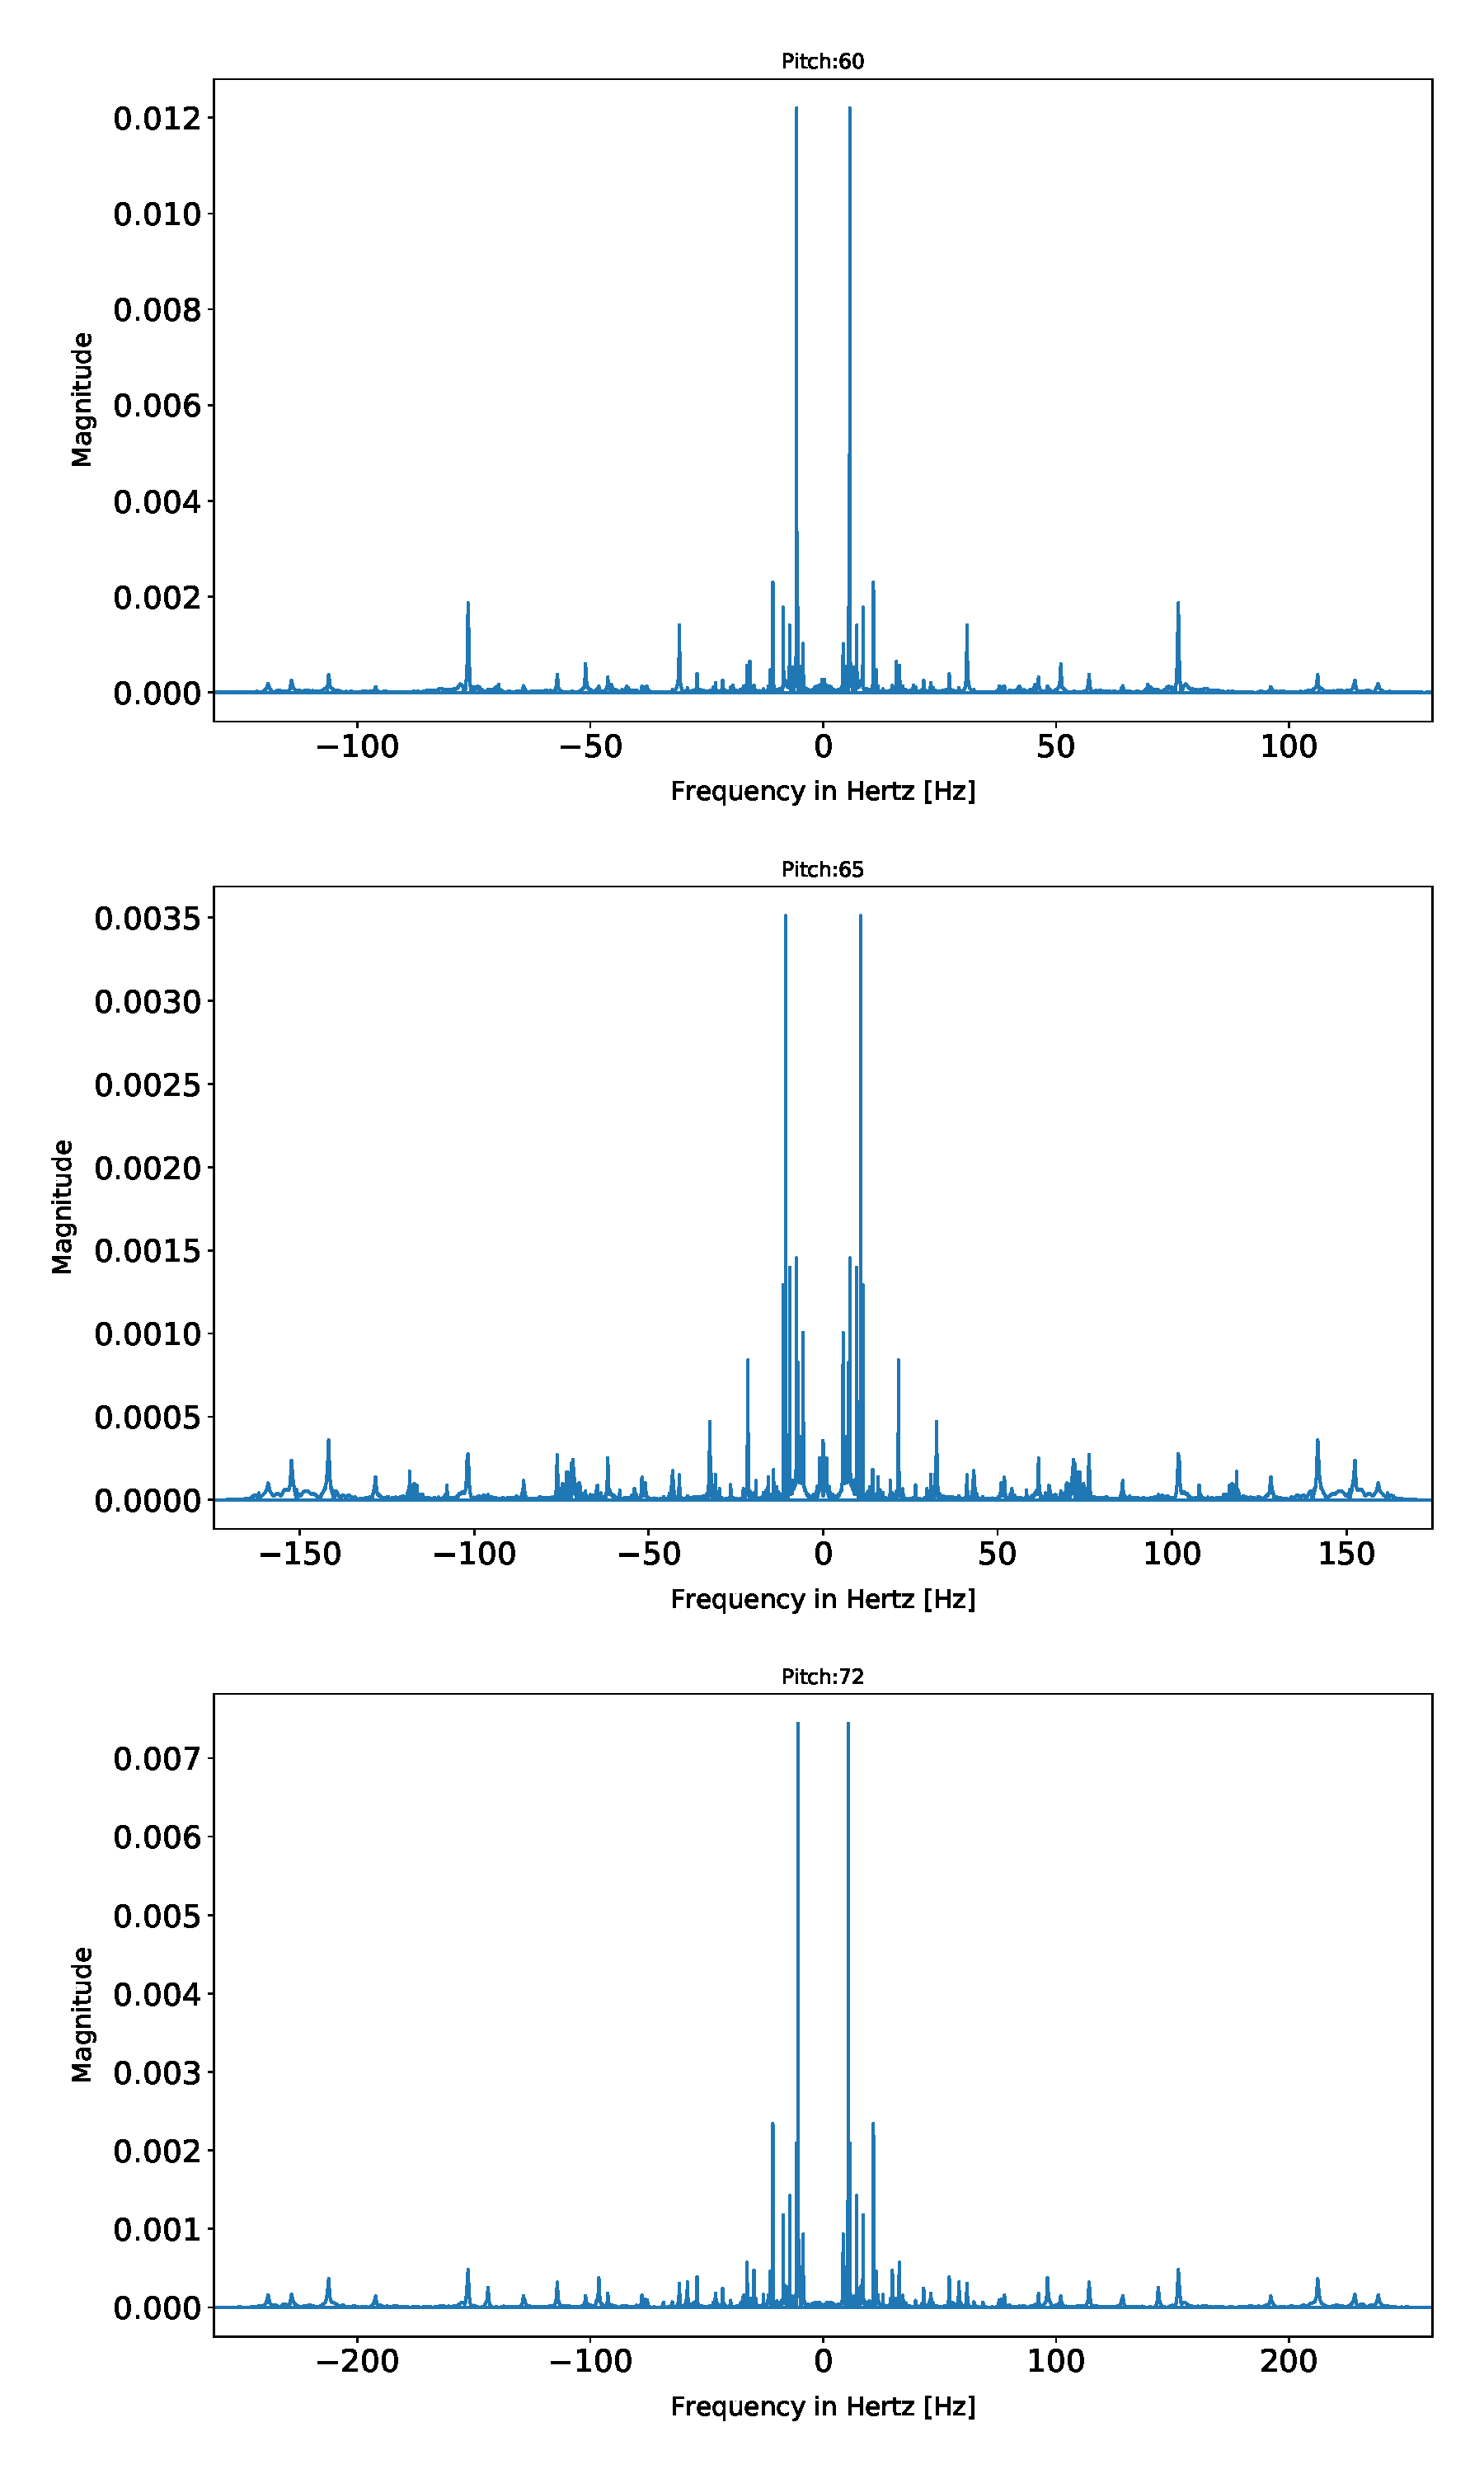
\includegraphics[width=200pt]{code/musicdata/pitch_classification.pdf}
		\caption{Pitch classification, coefficients of the logistic regression models for pitches $60$, $65$ and $70$.}
	\end{figure}

      
    \end{enumerate}
  \end{enumerate}

 \end{enumerate}
\end{document}
